% YZM411 Bilgisayarlı Görü -- Ödev 1 raporu (Overleaf, pdfLaTeX)
% Derleyici: pdfLaTeX (Overleaf varsayılanı) ya da XeLaTeX. Şekiller figures/ klasöründedir.
\documentclass[9pt,a4paper]{extarticle}

% ---- Öğrenci bilgileri ----
\newcommand{\ogrenciadi}{Muhammed Emin Erdağ}
\newcommand{\ogrencino}{230212013}

\usepackage{iftex}
\ifPDFTeX
  \usepackage[T1]{fontenc}
  \usepackage[utf8]{inputenc}
  \usepackage{newtxtext,newtxmath}
\else
  \usepackage{newtxmath}
  \usepackage{fontspec}
  \setmainfont{texgyretermes}[Extension=.otf,UprightFont=*-regular,BoldFont=*-bold,ItalicFont=*-italic,BoldItalicFont=*-bolditalic]
\fi
\usepackage[turkish,shorthands=off]{babel}
\usepackage{icomma}
\usepackage[a4paper,top=10mm,bottom=10mm,left=13mm,right=13mm]{geometry}
\usepackage{graphicx}
\usepackage[table]{xcolor}
\usepackage{tabularx,booktabs,array}
\usepackage{enumitem}
\usepackage{multicol}
\setlength{\multicolsep}{1pt}
\usepackage{titlesec}
\usepackage[hidelinks]{hyperref}

\pagestyle{empty}
\setlength{\parindent}{0pt}
\setlength{\parskip}{0.5ex}
\linespread{1.0}

% Bölüm başlıkları: küçük, kalın, alt çizgili
\titleformat{\section}{\normalfont\fontsize{10.5}{12.5}\selectfont\bfseries}{}{0pt}{}[{\color{black!45}\titlerule[0.4pt]}]
\titlespacing*{\section}{0pt}{1.1ex}{0.5ex}

% Yardımcı komutlar
\definecolor{kirmizi}{HTML}{AA0000}
\definecolor{yesil}{HTML}{006600}
\newcommand{\anah}[1]{\textbf{#1}}                        % anahtar söz
\newcommand{\kotu}[1]{\textcolor{kirmizi}{\textbf{#1}}}   % tutmayan tahmin
\newcommand{\iyi}[1]{\textcolor{yesil}{\textbf{#1}}}      % tutan tahmin
\newcommand{\kod}[1]{\texttt{\small #1}}
\newcommand{\kucuk}{\fontsize{8}{9.5}\selectfont}
\newcommand{\sekilnotu}[1]{\par\vspace{0.3ex}{\kucuk\textcolor{black!75}{#1}}\par\vspace{0.4ex}}
\newcolumntype{R}{r}
\newcolumntype{Y}{>{\raggedright\arraybackslash}X}
\setlength{\tabcolsep}{3pt}
\renewcommand{\arraystretch}{1.08}
\newenvironment{sutun}[1]{\begin{minipage}[t]{#1}\setlength{\parskip}{0.5ex}}{\end{minipage}}
\setlist[itemize]{leftmargin=4mm,itemsep=0.1ex,topsep=0.2ex,parsep=0pt}

\begin{document}
\fontsize{9.3}{11.2}\selectfont

{\fontsize{14}{17}\selectfont\bfseries YZM 411 Bilgisayarlı Görü --- Ödev 1: Renk, Aydınlatma ve Örnekleme\par}
\vspace{0.4ex}
{\fontsize{8.5}{10.5}\selectfont\textcolor{black!80}{\textbf{Öğrenci:} \ogrenciadi\ \ $|$\ \ \textbf{No:} \ogrencino\ \ $|$\ \ \textbf{Kod:} \kod{odev1.ipynb}\ \ $|$\ \ \textbf{Ham sonuçlar:} \kod{results/*.csv}, \kod{results/olcumler.json}}\par}
\vspace{0.6ex}

\anah{Sahne ve çekim.} Hedef nesne turuncu kumaş kalemlik. Yanında beyaz A4 kâğıt, küçük puntolu yazısı olan bir iskambil kartı, sarı-mor bir kitap ve içinde turuncu çay olan bir kupa var; masa çizgili ahşap.
Üç fotoğraf Samsung Galaxy A54 ile 10\,s arayla çekildi: normal oda ışığı, gölge (sahneye düşen ışık engellendi) ve sıcak renkli masa lambası.
EXIF'e göre \textbf{otomatik pozlama ve otomatik beyaz dengesi açıktı}. Pozlama süresi $\times$ ISO, normale göre gölgede \textbf{2,64$\times$}, lambada 0,80$\times$ oldu. Bu yüzden \textbf{``yalnızca ışık değişti'' diyemiyorum}: kamera kazancı ve renk dengesi de değişti.
Telefon çekimler arasında biraz kaydı. Gölge ve lamba fotoğraflarını normale SIFT~[5] + RANSAC~[6] homografisiyle hizaladım (ölçek 1,018 / 1,036; ortanca hata 0,96 / 0,86\,px). Hizalamada \kod{INTER\_NEAREST} kullandığım için yeni renk değeri üretilmedi. Alan oranlarını üç fotoğrafın ortak görüş alanı (karenin \%99,8'i) üzerinden hesapladım.

\vspace{0.4ex}
\noindent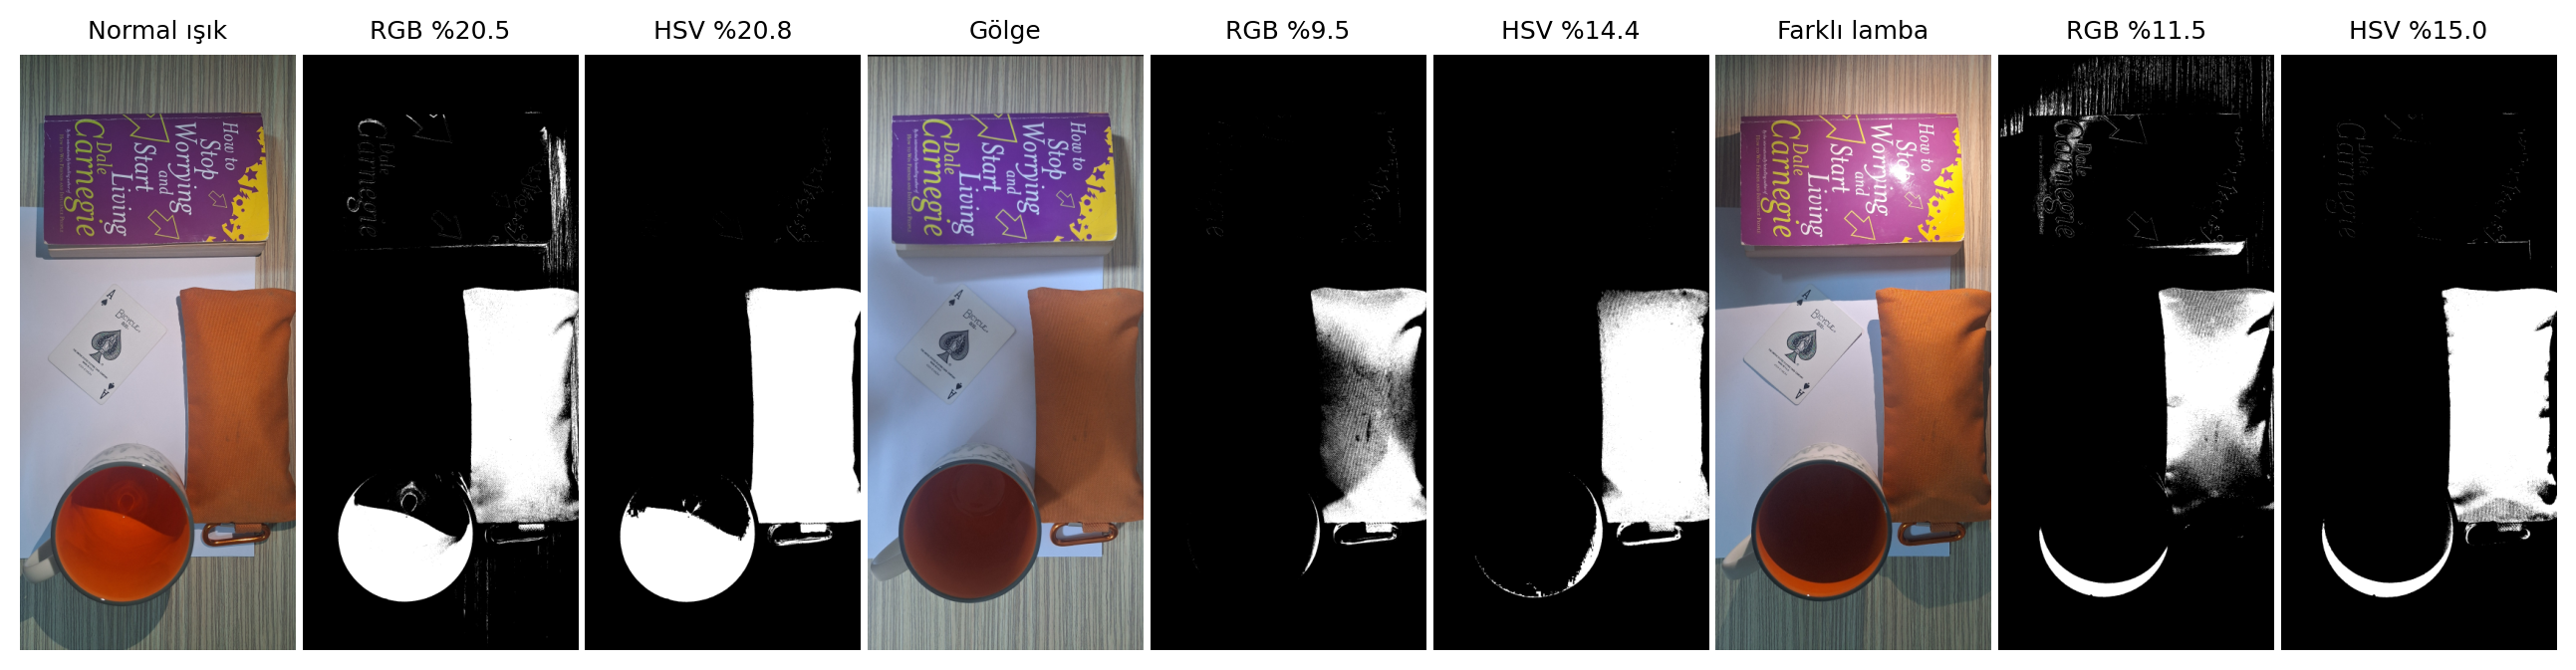
\includegraphics[width=\linewidth]{figures/fig5_rapor_foto_maske.png}
\sekilnotu{\textbf{Şekil 1.} Üç özgün fotoğraf (hizalanmış) ve aynı dondurulmuş eşiklerle elde edilen altı maske. Başlıktaki yüzde, maskenin ortak görüş alanına oranıdır (doğruluk değildir).
Eşikler normal ışıktaki 250$\times$250\,px kalemlik bölgesinin \%2--98 aralığından türetildi ve \textbf{bir kez dondurulup değiştirilmedi}: \textbf{RGB} R 115--230, G 30--145, B 0--95; \textbf{HSV}~[4] H 5--16, S $\geq$ 125, V $\geq$ 80 (OpenCV~[8], H 0--179).}

\noindent
\begin{sutun}{0.465\linewidth}
\section*{1. Sayısal yapı (H1)}
\kod{img.shape = (4080, 1884, 3)}, \kod{uint8}, değer aralığı 0--255. Erişim \kod{img[y, x, kanal]} şeklinde: P1 için \kod{img[1850, 1250]} OpenCV'de (B, G, R) = (35, 74, 159) verdi; \kod{cvtColor(BGR2RGB)} sonrası (159, 74, 35). \kod{img[x, y]} yazınca başka bir piksel okundu.

{\kucuk
\begin{tabularx}{\linewidth}{@{}Ylll@{}}
\toprule
\textbf{Piksel (x, y), 5$\times$5 ort.} & \textbf{Normal (R,G,B)} & \textbf{Gölge} & \textbf{Lamba} \\
\midrule
P1 (1250, 1850) & 165, 80, 40 & 132, 77, \textbf{62} & 195, 107, 55 \\
P2 (1650, 2300) & 140, 66, 27 & 108, 60, \textbf{38} & 124, 60, 28 \\
P3 (1400, 2900) & 134, 60, 25 & 111, 61, \textbf{39} & 115, 57, 31 \\
\bottomrule
\end{tabularx}\par}

\anah{Tahmin:} Gölgede R, G ve B birlikte düşecek; sıcak lambada B orantısız düşecek.
\anah{Ölçüm:} Gölgede R düştü, G yaklaşık sabit kaldı, \textbf{B arttı}. Lambada P1'de üç kanal da arttı, P2 ve P3'te R ve G biraz düştü; kalemliğin ortanca rengi (175, 87, 41) $\rightarrow$ (171, 88, 41) ile neredeyse aynı kaldı. \kotu{İki tahmin de tutmadı.}

\anah{Ne gördüm / neden / kontrol:} Gölgedeki yüzey doğrudan ışık yerine mavimsi dağınık ortam ışığıyla aydınlanıyor; kamera da kazancı 2,64$\times$ artırarak karanlığı kısmen telafi etti. Lambada otomatik beyaz dengesi sıcak ışığı nötrledi; geriye yalnızca konuma bağlı parlaklık farkı kaldı (lamba sol üstte: P1 1,25$\times$, P2 0,91$\times$).
\textit{Kontrol:} Pro modda ISO, enstantane ve WB kilitli olarak yeniden çekip aynı pikselleri ölçmek.
\end{sutun}\hfill
\begin{sutun}{0.515\linewidth}
\section*{2. Sabit RGB / HSV eşikleri (H2)}
{\kucuk
\begin{tabularx}{\linewidth}{@{}llRRY@{}}
\toprule
\textbf{Foto.} & \textbf{Uzay} & \textbf{Alan} & \textbf{Ref. kaps.} & \textbf{Seçimlerin geldiği yer} \\
\midrule
Normal & RGB & \%20,54 & \%100 & kalemlik \%67, \textbf{çay \%27} \\
Normal & HSV & \%20,78 & \%100 & kalemlik \%72, \textbf{çay \%26} \\
Gölge  & RGB & \%9,46  & \textbf{\%57,8} & kalemlik \%98 \\
Gölge  & HSV & \%14,38 & \%100 & kalemlik \%96 \\
Lamba  & RGB & \%11,46 & \%99,8 & kalemlik \%78, çay \%9, \textbf{kitap \%7, ahşap \%5} \\
Lamba  & HSV & \%15,04 & \%100 & kalemlik \%92, çay \%7, ahşap \%0 \\
\bottomrule
\end{tabularx}\par}

\anah{Tahmin:} Gölgede RGB maskesi küçülecek, HSV ton kanalı sayesinde daha az etkilenecek; lambada açık renkli yüzeyler eşiği geçecek.
\anah{Ölçüm:} Gölgede RGB maskesi \%20,5'ten \%9,5'e düştü ve referans bölgenin yalnızca \%58'ini seçti; HSV \%100 kapsamayı korudu. \iyi{Tuttu.}
Lambada kâğıt değil, \textbf{ahşap ve kitap} eşiği geçti, o da yalnızca RGB'de. \anah{Kısmen tuttu.}

\anah{Ne gördüm / neden:} Gölgede kalemliğin ortancası (175, 87, 41) $\rightarrow$ (117, 65, 43) oldu; R alt eşik 115'e dayandı. HSV'de ton sabit kaldı (H 10 $\rightarrow$ 9), ama S 195 $\rightarrow$ 162'ye, P1 pikselinde 132'ye indi. Bu değer S $\geq$ 125 sınırına çok yakın: \textbf{HSV'yi yalnızca bıraktığım pay kurtardı}, HSV her aydınlatma değişimine dayanıklı değil.
HSV alanının \%20,8'den \%14,4'e düşüşünün çoğu kalemlikten değil, gölgede karardığı için seçilmeyen \textbf{çaydan} geliyor: yalnızca kalemlik kutusunda HSV oranı \%14,9 $\rightarrow$ \%13,8. Alan oranı doğruluk değildir.
\textit{Kontrol:} S ve V alt eşiklerini değiştirip HSV kapsamının hangi değerde çöktüğünü ölçmek; çayı ayırmak için şekil ölçütü (en--boy oranı, doluluk) eklemek.
\end{sutun}

\section*{Soru 1: ``Sarı bir arka plan neden hedef gibi seçildi?''}
Kamera nesneyi değil, ondan yansıyan ışığı ölçer. Lambada normalde griye yakın olan ahşap (H 42, S 23) sıcak ışıkla turuncumsuya döndü (H 12, S 61).
RGB eşiği her kanalı ayrı ayrı sınırlar ve ``ne kadar renkli'' olduğunu sormaz; bu yüzden soluk turuncu ahşabın 40\,885 pikseli (ortanca 124, 102, 92) kutunun içine düştü. Kitaptaki sarı-turuncu bölgeler de aynı şekilde seçildi. HSV'deki S $\geq$ 125 koşulu bu solukluğu reddetti.
Normal ışıkta ise çay (H 7) kalemlikle (H 10) gerçekten aynı tonda olduğu için iki uzayda da seçildi. Eşik \textbf{renkli bölgeyi} bulur, \textbf{nesneyi} değil.

\section*{Sınırlar}
\begin{itemize}
\item Otomatik pozlama ve beyaz dengesi açıktı; her koşulda yalnızca bir fotoğraf var, bu yüzden sonuçlar istatistiksel değil, gözlemseldir.
\item Gölge sahneye tam homojen düşmedi; elle çizilen bölgeler (\kod{REGIONS}) ve hizalama $\pm$1\,px hata içerir; JPEG sıkıştırması da renkleri hafifçe değiştirir.
\item Maske alan oranı ve bölge payları ``eşiği geçen piksel'' ölçüsüdür; nesne tespit doğruluğu olarak yorumlanmamalıdır.
\end{itemize}

\newpage

\noindent
\begin{sutun}{0.47\linewidth}
\section*{3. Parlaklık ve gama (H3)}
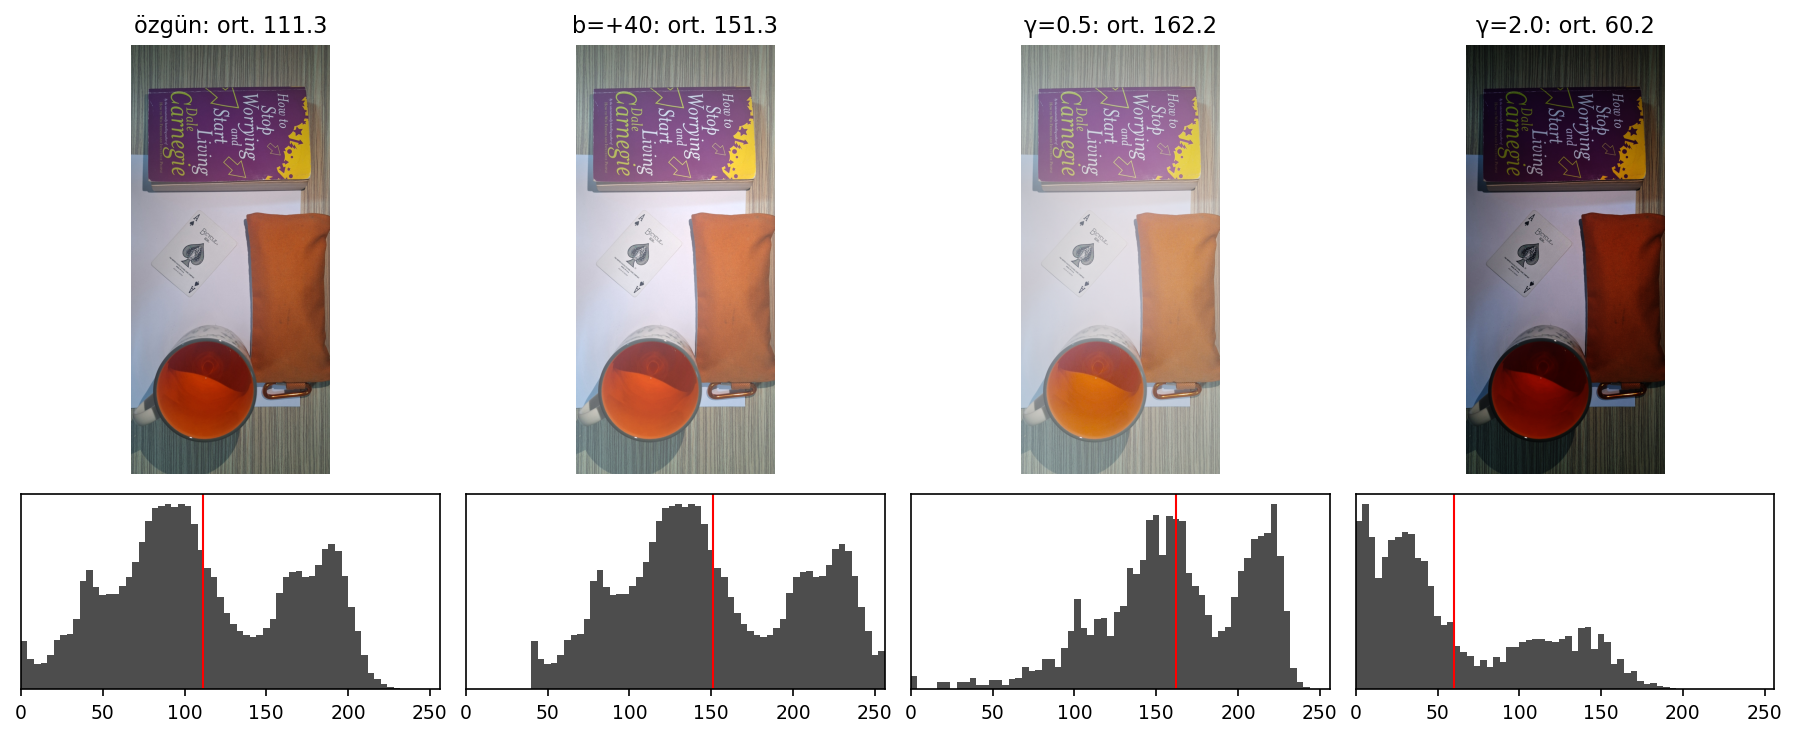
\includegraphics[width=\linewidth]{figures/fig3_parlaklik_gama.png}
\sekilnotu{\textbf{Şekil 2.} $J = \mathrm{clip}(I + 40)$ ve $J = 255\cdot(I/255)^{\gamma}$; dönüşümler float üzerinde yapıldı, [0, 255]'e kırpıldı, yuvarlandı. Kırmızı çizgi ortalamayı gösterir.}

{\kucuk
\begin{tabularx}{\linewidth}{@{}YRRR@{}}
\toprule
\textbf{Dönüşüm} & \textbf{Ön tahmin (ortalama)} & \textbf{Ölçülen} & \textbf{255 olan değer} \\
\midrule
Özgün            & ---    & 111,32 & \%0,01 \\
$b = +40$        & 151,32 & 151,30 & \%0,46 \\
$\gamma = 0{,}5$ & 168,49 & 162,22 & \%0,01 \\
$\gamma = 2{,}0$ & 48,60  & 60,22  & \%0,01 \\
\bottomrule
\end{tabularx}\par}

\anah{Tahmin:} +40 kaydırması 255'te kırpılma yüzünden ortalamayı 40'tan az artıracak ve en çok beyaz kâğıt kırpılacak. Gama sonrası ortalama $\approx 255\cdot(m/255)^{\gamma}$ olacak.
\anah{Ölçüm:} Artış +39,98 oldu; 215'i aşıp kırpılan kanal değerlerinin oranı yalnızca \%0,39. \kotu{Tahmin tutmadı.} Gamada yön doğru çıktı, ama ortalama tahminden $-$6,3 ve +11,6 saptı. \kotu{Tutmadı.} Tek değer kontrolü beklendiği gibi: 64 $\rightarrow$ 127,7 ($\gamma = 0{,}5$) ve 16,1 ($\gamma = 2{,}0$).

\anah{Neden / kontrol:} Otomatik pozlama beyaz kâğıdı bile $\sim$190'da (V ortancası 191) tuttuğu için +40 neredeyse hiç kırpılmadı. Gama doğrusal olmadığı için ortalamanın gaması, gamaların ortalamasına eşit değil (Jensen eşitsizliği): içbükey $\gamma = 0{,}5$'te ortalama tahminin altında, dışbükey $\gamma = 2$'de üstünde kalır.
Tahmini tek bir ortalama yerine tüm piksel dağılımı üzerinden yeniden hesapladım: \kod{mean(min(I+40,255)) = 151,30} ve $\mathrm{mean}(255\cdot(I/255)^{\gamma}) = 162{,}24 / 60{,}24$; ikisi de ölçümle örtüşüyor.
\end{sutun}\hfill
\begin{sutun}{0.51\linewidth}
\section*{4. 1/4 küçültme (H4)}
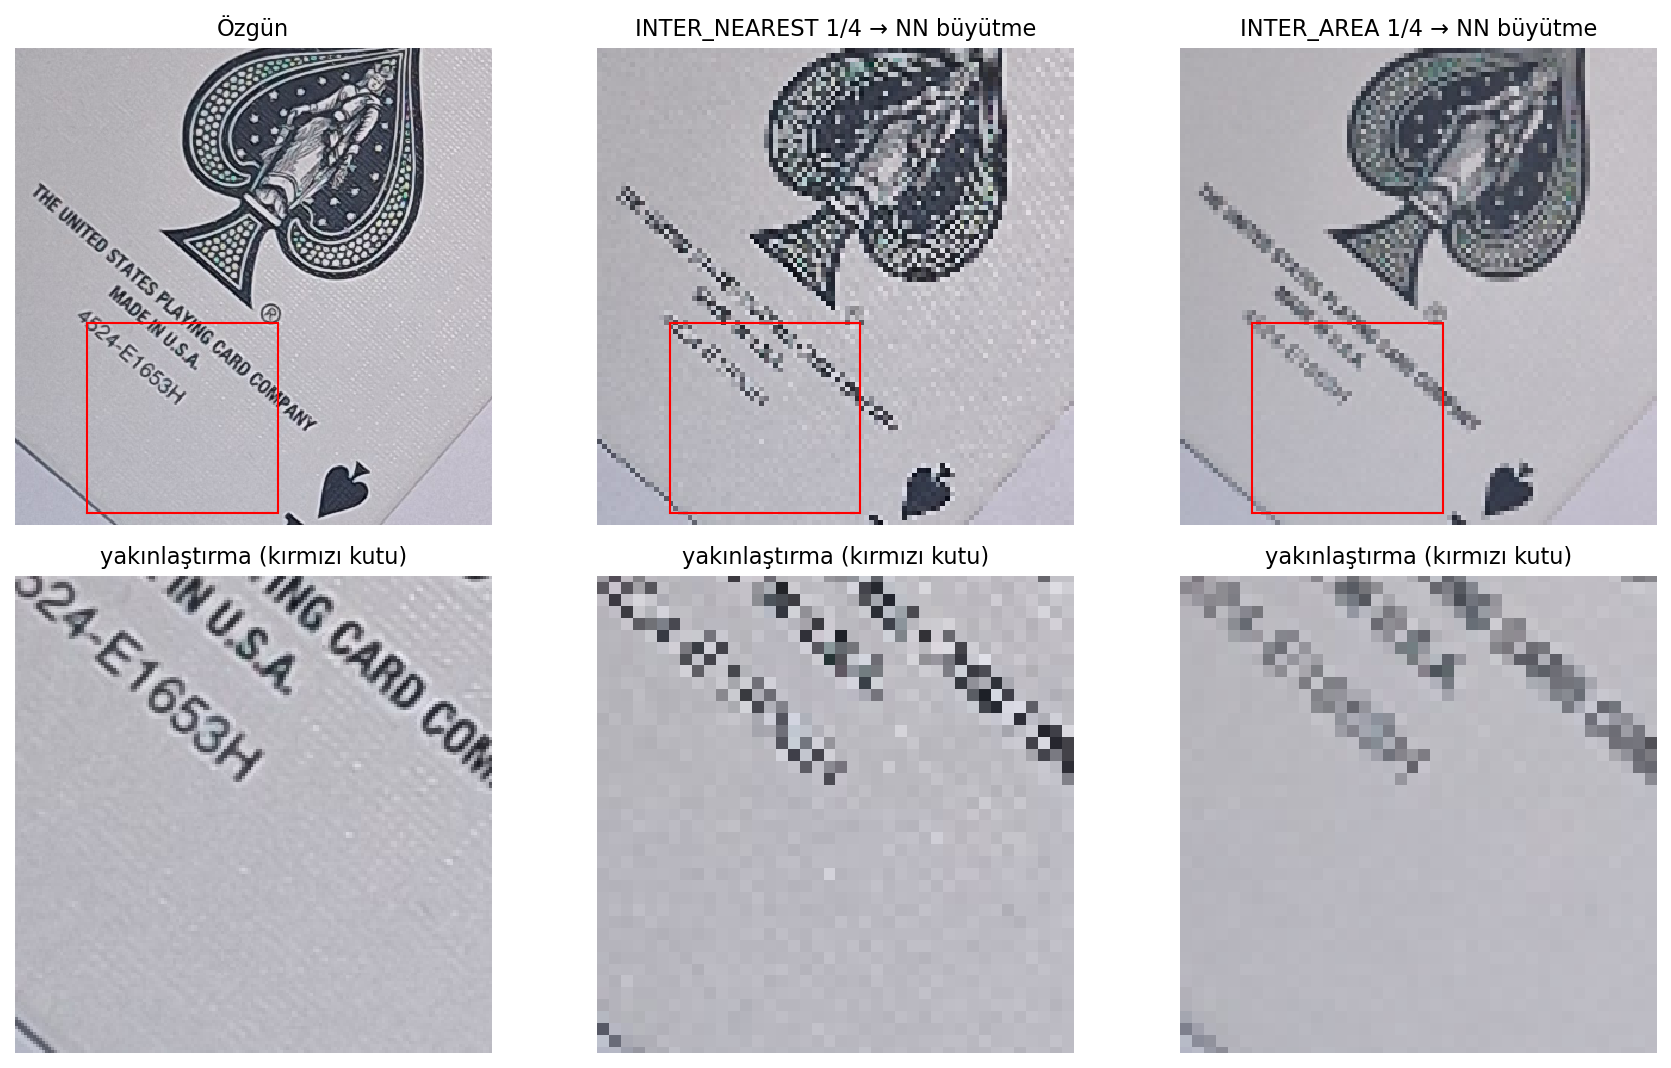
\includegraphics[width=\linewidth]{figures/fig4_kucultme.png}
\sekilnotu{\textbf{Şekil 3.} Karttaki 400$\times$400\,px kesit; \kod{INTER\_NEAREST} ve \kod{INTER\_AREA} ile 100$\times$100'e küçültüldü, yalnızca gösterim için en yakın komşuyla geri büyütüldü. Alt satır: ``MADE IN U.S.A.'' yakın planı.}

\anah{Tahmin:} Harfler 2--3\,px'e inip okunamayacak. NEAREST çizgileri koparıp sahte desen, AREA gri/bulanık yazı üretecek. Büyütme ayrıntıyı geri getirmeyecek.
\anah{Ölçüm:} Harf yüksekliği $\approx$ 12 $\rightarrow$ 3\,px; yazı iki yöntemde de okunamıyor. NEAREST, kartın ince keten dokusunu çapraz damalı \textbf{sahte bir desene} çevirdi; küçük görüntünün Laplace varyansı AREA'nınkinin 3,3 katı (keskinlik değil, örtüşme). AREA dokuyu sildi ve yazıyı griye çevirdi: mürekkebin en koyu \%1'lik değeri 31 $\rightarrow$ 49, kontrast (std) 48,6 $\rightarrow$ 41,4. \iyi{Tuttu.}

\section*{Soru 2: ``Büyütme kaybolan yazıyı neden geri getirmedi?''}
1/4 örneklemede temsil edilebilen en yüksek frekans (Nyquist sınırı~[2]) 0,125 devir/pikseldir; kesitteki enerjinin \textbf{\%21,6'sı} bu sınırın üstündeydi ve 160\,000 pikselden 10\,000'i kaldı.
En yakın komşu büyütmesi her pikseli 4$\times$4 blok olarak kopyalar, yeni bilgi eklemez. PSNR: NEAREST $\rightarrow$ NN 16,1\,dB, AREA $\rightarrow$ NN 20,0\,dB, AREA $\rightarrow$ bikübik 20,5\,dB. Bikübik yalnızca blok kenarlarını yumuşatıyor; harf ayrıntısı küçük görüntüde hiç olmadığı için geri gelmiyor. \textit{Kontrol:} NEAREST'ten önce Gauss bulanıklığı uygulayıp sahte desenin kaybolduğunu ölçmek; 1/2 ve 1/3 oranlarında okunabilirlik sınırını bulmak.
\end{sutun}

\section*{Tahmin -- ölçüm özeti (\kod{results/sonuc\_tablosu.csv})}
{\kucuk
\begin{tabularx}{\linewidth}{@{}l>{\raggedright\arraybackslash}p{0.27\linewidth}Yl@{}}
\toprule
\textbf{Deney} & \textbf{Tahmin} & \textbf{Ölçüm} & \textbf{Tuttu mu?} \\
\midrule
H1 & Gölgede R, G, B birlikte düşer & P1 (165,80,40) $\rightarrow$ (132,77,62): R$\downarrow$, G$\approx$, B$\uparrow$ & \kotu{Tutmadı} \\
H1 & Sıcak lambada B orantısız düşer & Kalemlik ortancası (175,87,41) $\rightarrow$ (171,88,41) & \kotu{Tutmadı (oto. WB)} \\
H2 & Gölgede RGB küçülür, HSV daha az & RGB \%20,5 $\rightarrow$ \%9,5 (ref. \%58); HSV \%20,8 $\rightarrow$ \%14,4 (ref. \%100) & \iyi{Tuttu} \\
H2 & Lambada açık yüzeyler eşiği geçer & RGB'de ahşap \%4,7 + kitap \%6,9; HSV'de ahşap \%0 & Kısmen \\
H3 & +40 artışı 40'tan az olur (kırpma) & 111,32 $\rightarrow$ 151,30; kırpılan \%0,39 & \kotu{Tutmadı} \\
H3 & Ortalama $\approx 255\cdot(m/255)^{\gamma}$ & 168,5 $\rightarrow$ 162,2 ($\gamma=0{,}5$); 48,6 $\rightarrow$ 60,2 ($\gamma=2$) & \kotu{Tutmadı (yön doğru)} \\
H4 & Harfler 2--3\,px olur, okunmaz & 12 $\rightarrow$ 3\,px, okunamıyor & \iyi{Tuttu} \\
H4 & NEAREST sahte desen, AREA gri yazı & Damalı doku deseni; en koyu \%1: 31 $\rightarrow$ 49 & \iyi{Tuttu} \\
H4 & Büyütme ayrıntıyı geri getirmez & PSNR 16,1 / 20,0 / 20,5\,dB; kayıp enerji \%21,6 & \iyi{Tuttu} \\
\bottomrule
\end{tabularx}\par}

\section*{Kaynaklar}
{\fontsize{7.6}{9}\selectfont
\begin{multicols}{2}
\begin{enumerate}[label={[\arabic*]},leftmargin=5mm,itemsep=0.1ex,topsep=0pt,parsep=0pt]
\item YZM411 Bilgisayarlı Görü, Hafta 1--2 ders notu.
\item R.\,C. Gonzalez, R.\,E. Woods, \textit{Digital Image Processing}, 4. baskı, Pearson, 2018.
\item R. Szeliski, \textit{Computer Vision: Algorithms and Applications}, 2. baskı, Springer, 2022.
\item A.\,R. Smith, ``Color gamut transform pairs,'' \textit{SIGGRAPH Comput. Graph.}, 12(3):12--19, 1978.
\item D.\,G. Lowe, ``Distinctive image features from scale-invariant keypoints,'' \textit{IJCV}, 60(2):91--110, 2004.
\item M.\,A. Fischler, R.\,C. Bolles, ``Random sample consensus,'' \textit{Commun. ACM}, 24(6):381--395, 1981.
\item N. Otsu, ``A threshold selection method from gray-level histograms,'' \textit{IEEE Trans. SMC}, 9(1):62--66, 1979.
\item OpenCV belgeleri, docs.opencv.org: \kod{cvtColor}, \kod{inRange}, \kod{resize}, \kod{SIFT}, \kod{findHomography}.
\item C.\,R. Harris vd., ``Array programming with NumPy,'' \textit{Nature}, 585:357--362, 2020.
\end{enumerate}
\end{multicols}}

\section*{Araç ve yapay zekâ beyanı (ödev madde 8.e)}
\textbf{Araç:} Claude (Anthropic), Claude Code ortamında. \textbf{Kullanım amacı:} \kod{odev1.ipynb} defterindeki kod hücrelerinin (yükleme, hizalama, maskeler, dönüşümler, küçültme, tablolar) ve deney yorumlarının ilk taslağının yazılması, eşik türetme yönteminin önerilmesi, rapor ve \kod{README.md} taslağının hazırlanması.
\textbf{Etkilediği dosyalar:} \kod{odev1.ipynb}, \kod{odev1.py}, rapor (\kod{main.tex} / PDF), \kod{README.md}.
\textbf{Doğrulama:} Defter yeniden başlatılıp baştan sona çalıştırıldı. Rapordaki her sayı \kod{results/} altındaki CSV/JSON dosyalarıyla karşılaştırıldı, şekiller fotoğraflarla gözle kontrol edildi. Fotoğrafları kendim çektim ve sahneyi kendim kurdum.

\end{document}
